The goal of this work is to understand which transformations are necessary to convert a program from a sequential programming model with shared memory into a distributed, concurrent programming model of a microkernel operating system. A significant part of these transformations is already implemented in the Ohua compiler. Therefore, the specific goal is to understand and close the 'translation gaps' between the programming models of the source program, the current Ohua implementation, and the M3 operating system. So to better understand the work that need to be done, we will introduce those models in this chapter.

\section{Ohua}
\label{sec:back_ohua}
In this section we will introduce the Ohua compiler\cite{ertel2015ohua}. Its essential concept is to extract the underlying data flow graph from a sequential input program. The result is a program structure consisting of individual steps that are connected only by incoming and outgoing data and can be executed concurrently. These individual steps and their data channels can then be mapped to various abstractions of processes and communication channels in the backend of the compiler to achieve parallelization and isolation of the steps. Like most compilers, Ohua works step-by-step with different intermediate representations (IRs) of the input program. In the next subsection, we will take a closer look at the basic structure and function of Ohua. For this work, it is also important to understand what programming model Ohua currently supports. Here, programming model means on the one hand which restrictions in the syntax of the input programs are currently necessary to be able to convert them into correct concurrent programs. On the other hand it contains the explicit and implicit assumptions about the concrete implementations of 'processes' and 'channels'. We will therefore also look at these aspects in more detail in this section.

\subsection{Compiler Pipeline}
When we say 'Ohua compiles a program', we mean it compiles functions in the compile scope. In contrast to e.g. rustc or gcc Ohua does not compile the complete code of the program, but transforms only the functions e.g. within one or more Python modules specified in the call. We call these functions algorithms. In contrast to algorithms, functions and methods that are imported and used within algorithms are not compiled. They are completely opaque to the compiler. This also means that Ohua does not require any syntax constraint in these imported functions and methods. An overview of the compiler pipeline is shown in Figure~\ref{fig:ohua_fine}.  

In the \textbf{compiler frontend}, algorithms of the target language are first parsed and translated into Ohua's frontend language (Frontend IR). This translation is implemented in language specific frontend integrations. That is, for each language supported by Ohua, such a frontend integration must exist. This integration parses algorithms of the input language and translates them into the syntax of the frontend IR. For non-supported syntax constructs, currently for example \code{break} statements in loops, the compilation terminates at this point. 

\begin{figure}[H]
    \centering
    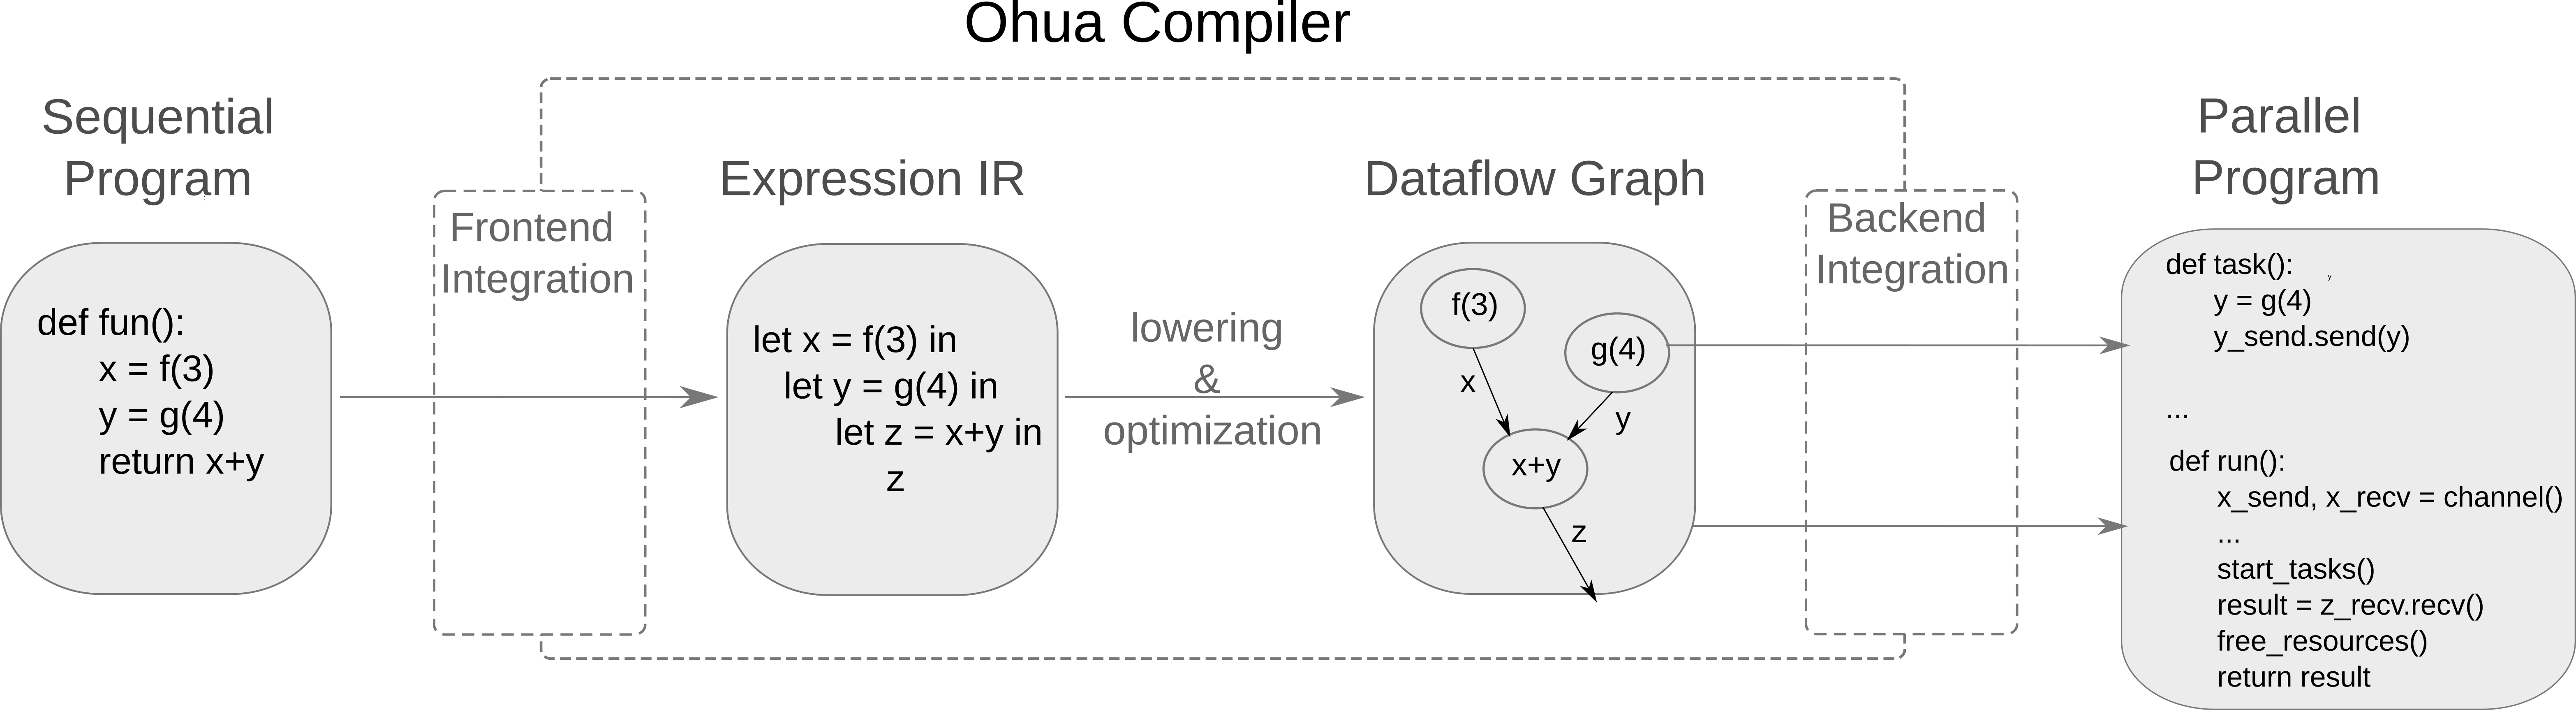
\includegraphics[scale= 0.36]{figures/ohua_fine_with_channels.png}
    \caption{Structural overview of Ohua and the code transformations}
    \label{fig:ohua_fine}
\end{figure}

In the \textbf{core compiler} itself there are two main representations of the code. One is Expression IR. This language is functional and based on the call-by-need lambda calculus. To transform input algorithms to this representation 
calls to other algorithms are inlined, renaming compiler passes ensure single static assignment form and assignment expressions are refactored to applicative normal form. A simplified example of code before and after the transformation is shown in Figure~\ref{fig:funBodyTranslation}. A central conversion step in the compiler is the transformation of stateful calls to so called \emph{state threads}(\cite{wadler1992essence}, \cite{launchbury1994lazy},\cite{ertel2019stclang}). To generate race condition free tasks, Ohua forbids shared state use and only permits stateful computation inside methods. However, methods in an imperative language mutate objects in place and implicitly refer to the new, changed state by the same reference as before. The conversion of stateful calls to state threads makes the semantic of creating a new state upon calling methods explicit. In the code example in Fig.\ref{fig:funBodyTranslation}, the call \rust{someState.do()}, is internally transformed to explicitly take a state as an argument and return a new, mutated state. Thereby, function calls downstream to not need to access a shared memory to use stateful objects. Based on this explicit state threading, Ertel et al. \cite{ertel2019stclang, ertel2018supporting} developed functional representations for imperative control flow on stateful computations. For example an imperative for-loop, is translated to a so called \code{smap} operation, which is essentially a fold operation of the loop body on the states manipulated inside the loop.  


\begin{figure}
    \centering
    \begin{subfigure}[b]{0.45\textwidth}
         \centering
         \begin{minted}{rust}
 fn algo(i){
   let someState = 
           other_algo(i);
   let a = someState.do()
   let b = f(a)
   return b
 }

 fn other_algo(i){
    let s = State::new(i)
    s
 }
            \end{minted}
         \caption{Input algorithm}
         \label{simplPyInput}
     \end{subfigure}
     \hfill
     \begin{subfigure}[b]{0.5\textwidth}
         \centering
         \begin{minted}[escapeinside=||,mathescape=true]{haskell}
let someState = 
        |$\lambda$| State::new (i) in
  let a, someState_0 = 
           |$\lambda$| do (someState, a) in
    let b = |$\lambda$| f (a) in
        b
        \end{minted}
        \vspace{15mm}
    \caption{Pseudocode of IR}
         \label{simplIR}
    \end{subfigure}
\caption{An algorithm is mapped to a nested let-expression with the innermost term representing its return value}
\label{fig:funBodyTranslation}
\end{figure}

The next representation in the compile flow is the Data Flow Graph (DFG) representation. Independent program tasks are encapsulated in the this representation and are explicitly assigned their incoming outgoing data channels. Besides function calls from the original program, this representation also contains control nodes that govern the data flow. For example if the input code contained a branching statement like \rust{if cond {f()} else {g()}} control nodes will be introduced to a) switch data flow between calls to \code{f()} or \rust{g()} and b) to collect results from appropriate output channels of \code{f()} or \rust{g()} depending on the condition. This representation also allows to merge certain nodes by fusing their code, as well as input and output channels. This is done for instance if a following node entirely depends on its predecessor and has so little work to do, that it would hardly justify the overhead of spinning up an independent task in any backend implementation.\\

Which ultimately brings us to the \textbf{compiler backend} and backend integrations of Ohua. Backend integrations consist of two parts. The 'Language Backend' is only language specific. Similar to the frontend integration, it serves the purpose of translating code inside tasks from Ohua representation syntax back to the target language syntax. The 'Architecture Backend' is responsible for translating the 'nodes' and 'edges' of the DFG into a specific implementation for concurrent tasks, communication channels and a runtime for the graph. For example their can be two different architectures for a given language one implementing tasks as threads, one using processes both also generating appropriate channels and runtime code to execute the DFG. As we did not compile imported functions the target language must match the input language, which is automatically ensured by the compiler. Architectures for the same language can be used interchangeably. This way Ohua can generate e.g. multi-threaded shared memory or fully distributed programs from the same input.\\

In the next section we will take a closer look at the restrictions and assumptions required to make this work.

\subsection{Programming Model}

The term programming model generally describes a relationship between syntax constructs in a programming language and their concrete semantics in a particular execution environment. In the case of Ohua, the programming model includes, on the one hand, the supported input syntax and the assumptions made about the supported terms of the input language. On the other hand, it specifies how these terms are translated into a dataflow graph and what assumptions Ohua makes about the implementation of nodes, edges, and runtime of the DFG. First we will look into the supported input syntax and assumed semantics. 

\subsubsection{Input Syntax and Semantics}
We already know, that Ohua's basic input unit are algorithms, i.e. pure functions inside the compile scope. Figure~\ref{tab:FrontendIR} depicts the language definition of the frontend representation described before. Any syntax construct of the input language has to be mapped to the according terms of these language to be compiled. In the following paragraphs we will describe the accepted syntax constructs and the semantics the programming model expects them to have. \\


\begin{table}[ht]
\resizebox{\columnwidth}{!}{%
    \begin{tabular}{l c l l}
        \multicolumn{4}{l}{\emph{Patterns:}}\\
        $p$ & $::=$ & $x\ |\ (x,~\ldots ,~x)\ |\ ()$ & named variables, tuples or unit\\
        \multicolumn{4}{l}{\emph{Expressions:}}\\
        $e$ & $::=$ & $e$ & named expression in host language\\
        & $|$ & $\textbf{1},\textbf{2},\textbf{3}, \ldots \ |\ \textbf{true}\ |\ \textbf{false}\ |\ \textbf{()} $ & typed literal in host language\\
        & $|$ & $\textbf{let}\ p\ \textbf{=}\ e\ \textbf{in}\  e$ & lexical scoping \\
        & $|$ & $e\ e$ & application\\
        & $|$ & $\boldsymbol{\lambda} [p,~\ldots ,~p]\textbf{.}\  e$ & abstraction \\
        & $|$ & $\textbf{if}\ e\ \textbf{then}\ e\ \textbf{else}\ e$ & conditionals\\
        & $|$ & $\textbf{map}\ e\ e$ & map first expression to second\\
        & $|$ & $\textbf{bind}\ e\ e$ & bind an expression representing a state to  \\
        & & & an expression representing a function to act on this state \\
        & $|$ & $\textbf{stmt}\ e\ e$ & expression whose return value is ignored\\
        & $|$ & $\textbf{seq}\ e\ e$ & \\
        & $|$ & $\textbf{(}\ e\ \textbf{)}$ & tuple of expressions \\
    \end{tabular}%
    }
    \caption{}
    \label{tab:FrontendIR}
\end{table}

\textbf{Function Calls:} Beside algorithms, Ohua supports stateful and stateless function calls, i.e. methods and pure functions, imported into the scope. Pure functions are expected to be side effect free. In particular the programming model assumes, that pure functions do not implicitly manipulate their arguments. This excludes for instance functions that manipulate their arguments by reference. If the output of a pure function call is not used it is considered to have no effect and is removed during compilation. 

Stateful function calls on the other hand are expected to manipulate the object they are called on, i.e. have a side effect. Consequently they are not removed regardless if the output is used. 
Any stateful computation is expected to happen exclusively and explicitly using  method calls and also method calls are expected to only manipulate the object state itself. This also entails the requirement, that state is not 'leaked' via return values. For example in the method call \rust{let x = SomeState.do_stuff();}, \rust{x} must not be, or contain a reference to \rust{SomeState}. We already assumed, that other functions do not manipulate \rust{SomeState} when using \rust{x} as argument. However without this 'leaking assumption' it would be possible to call \rust{x} as a stateful object, thereby implicitly manipulating the state of \rust{SomeState}. This implicit semantic is not handled currently and would be lost in the distributed output code. 

Functions need to be typed or type-able by the frontend integration. To correctly annotate the types in generated code, at least to the extend required for any particular backend and architecture, Ohua needs to extract type information from the input code. Specifically the argument types of each function call are extracted and preserved in the different IRs as typed function literals capturing the argument types of each function call. 

\textbf{Loops}: Ohua supports bound and unbound \code{for}-loops. They are transformed into parallelizable pipelining of the independent calculation steps inside the loop. Inside for-loops each state from outside the loop must be used at most once to enable the accumulation of state changes in a single node for each object. Conditional loops (\code{while} or \code{do-while}) are as of the beginning of this work not supported, but can be expressed using recursion.

\textbf{Recursion}: Ohua supports recursion with some notable restrictions. Recursive algorithms must be tail recursive, the recursive call must be located in the if-branch, the return value must be in the else-branch of recursion. Further either one must be the only statement in each branch respectively. As return values only single variables are supported. Recursive loops will not yield any pipelining or parallelization but a loop executed for one input at a time. This is due to the semantic of recursion, being a repeated function on a state, where the result of each step depends not only on the step but also on previous results.
Currently the output of recursive algorithms can not be used in an assignment i.e. a recursive call can only be the last statement in another algorithm and return the calling algorithms final result. 

\textbf{Branching:} Branching is supported in case of simple if-else expressions, where both branches must be present. Also if-else statements as for instance present in the Python syntax are not supported currently. This is because in those statements have a different execution semantic than expressions i.e. branches that do not return a value but have side effects on variables from the surrounding scope. So they need to be implemented separately.

\textbf{Return, Continue, Break:} Ohua does currently not support any forms of early return of conditional execution except for recursion and branching as described before. Therefor \rust{break} and \rust{continue} are generally not supported at the moment, while \rust{return} is supported only for Python and only at as the last statement of a function block, because contrary to Rust there is no implicit value return in Python. 

\textbf{Variables and Literals:} There are two categories of variables. Local variables are bound inside algorithms, environment variables are bound in outer scope. So environment variables are basically arguments of the algorithms, but can also be imported or globally defined names. Ohua supports mutable and immutable local variable bindings. Local variables can either be used as a state, or as an argument to a function call. If it is used as an argument it can only be used once, if it is used as a state it may be used more than once, except, as explained before inside loops. Environment variables can not be used as a state directly\footnote{This changed during this work. Now arguments to algorithms can be used directly as a generator for a for-loop.}, but can be used several times as function call argument. The underlying assumption of this distinction is, that environment variables will be available in scope for all nodes created from an algorithm, while locally bound variables are send to the consuming node. This assumption becomes relevant in architectures, where the generated tasks have no access to a common global scope. In those cases, environment variables are not available to the task via a closure mechanism. This will be the case for M3 tasks. \\
Finally there is a limited set of literals that is directly supported in the input. This includes integers, booleans, strings and unit literals. Other literals must be wrapped in a function call currently, simple binary operations are sufficient here e.g. to compile \rust{let x = 17} one could write \rust{let x = 17 + 0}.

Many of the current limitations are only due to lack of implementation. For example, there is no formal reason to allow recursive calls only in the if branch. These limitations will be fixed in the future. At the moment, however, they are the main reason why control flow expressions cannot be freely combined. That is, there are currently restrictions on the frontend language that are not reflected in the language itself.

\todo[inline]{Give example code. If possible list restrictions and give explanation at least concerning the nature of restriction as a) immanent feature of the IR/Programming Model or b) Current lack of implementation}


\subsubsection{Enforcement}

Conformity with the allowed syntax subset is automatically implemented by each language integration, as it has to translate the input syntax to the frontend language. However, this is only a syntactical conversion. Except for tracking the annotated type of named variables, the compiler does no further semantic analysis of the input code. This means to comply with a programming model requirement it is sufficient to match the expected syntax, not necessarily the expected semantics. Take for example the requirement to use each variable only once as a function input. To use a variable \rust{x} twice, a programmer needs to return it twice from a function call \rust{let (x1, x2) = fun()}. However she can freely decide whether \rust{x1} and \rust{x2} are copies or only references of \rust{x}, matching the expected syntax but not the expected semantics of the programming model. The result might still be valid output but it is the responsibility of the programmer to ensure validity of reference passing in the concurrent output. Likewise, the use of global mutable state can be encapsulated in function calls. \\

In general enforcement of the programming model is currently not separately implemented and in some case lacking at all. Violations of the programming model will either lead to runtime errors during any point of compilation or may lead to invalid output code. The later case was not an obvious problem in Rust, as Rust itself enforces borrowing rules and therefore a considerable part of Ohuas limitations. However this is not generally the case in other languages, so tests where added in the course of this work to ensure compilation failure upon violations of the programming model.


\subsubsection{Backend Language and Process Abstractions}

The terms of Ohuas backend language are depicted in Table~\ref{tab:DFGdef}. As complex syntax constructs of the input laguage are removed in the frontend, most of the terms in the backend language are basic constructs of any imperative language, as variables, literals, assignments and simple control flow terms. To generate the code for Ohua introduced control nodes, some \emph{specific functions} are also required to be present in the host language. In particular the control of loop execution requires implementations for list handling, as well the functionality for \emph{interable objects} of the host language to test if they have a fixed size and if so retrieve this size information. 

Obviously the backend language also entails the notion of named and typed channels, their sending and receiving ends and sending and receiving of variables a means of communication among the tasks of the data flow graph. 

\begin{table}[ht]
\resizebox{\columnwidth}{!}{%
    \begin{tabular}{l c l l}
        \multicolumn{4}{l}{\emph{Typed Task Expressions:}}\\
        $e$ & $::=$ & $ x\ | \textbf{1}, \ldots \ |\ \textbf{true}\ |\ () $ & variables, simple literals \\
         & $|$& $ \textbf{funRef}\ | ref \textbf{envRef}\ !HostExpr  $ & function and environment references \\
        & $|$ & $ x (e,~\ldots,~e) |\ Obj.x (e,~\ldots,~e)  $ & pure function and method calls\\
        & $|$ & $\textbf{let} x\ \textbf{=}\ e\ \textbf{in}\ e |\ \textbf{=}\ e$ & scoped bindings and assignments \\
        & $|$ & $\textbf{stmt}\ e\ e$ & statement \\
        & $|$ & $x\textbf{\_receiver.receive()} $ & expression to  receive data \\
        & $|$ & $x\textbf{\_sender.send(}x\textbf{)} $ & expression to send data \\
        &\multicolumn{3}{l}{--control flow--}\\
        & $|$ & $\textbf{while True:}\ e$ & \\
        & $|$ & $\textbf{for}\ x\ \textbf{in}\ x\ \textbf{do}\ e$ & \\
        & $|$ & $\textbf{repeat}\ (x\ |\ l)\ e$ & \\
        & $|$ & $\textbf{while}\ e\ e$ & \\
        & $|$ & $\textbf{if}\ e\ \textbf{then}\ e\ \textbf{else}\ e$ & \\
        &\multicolumn{3}{l}{-- specific functions, required for control nodes --}\\
        & $|$ & $\textbf{newList}\ $ & create a list \\
        & $|$ & $\textbf{append}\ x\ e $ & append t to x \\
        & $|$ & $\textbf{hasSize}\ x$ & $[a]$ \means Bool \\
        & $|$ & $\textbf{size}\ x$ & $[a]$ \means Int \\
        & $|$ & $\textbf{(}\ l,\ l\textbf{)}\ | \  \textbf{(}\ x,\ x\textbf{)}$ & Tuple of literals or bindings\\
        & $|$ & $(x ,\  \_ )$ & First\\
        & $|$ & $(\_ ,\ x )$ & Second \\
        & $|$ & $ x++$ & Increment \\
        & $|$ & $ x--$ & Decrement \\
        & $|$ & $ \textbf{not}\ e$ & \\
        \multicolumn{4}{l}{\emph{Communication Channels:}}\\
        $channel\ $& $::$ &$\textbf{channel}\ x$& Typed channel, i.e. incoming and outgoing end for variable x\\
        & $|$ &$x\textbf{\_receiver}$& Typed receiving end of a  channel  \\
        & $|$ &$x\textbf{\_sender}$ &Typed sending end of a channel  \\
    \end{tabular}%
    }
    \caption{The terms of Ohuas backend language used to represent the DFG. Language specific backend integrations translate this language to generate the output program.}
    \label{tab:DFGdef}
\end{table}

A major advantage of compiling with Ohua is, that the generated dataflow-based language is deterministic. That is, a correct, deterministic, sequential program becomes a correct, deterministic, concurrent program by compilation. Formal verification of the compiler transformations to proof this claim and formalize the programming model is currently an ongoing task. Nevertheless, we can already clearly describe the assumptions concerning the concrete implementations of nodes, edges and the runtime each architecture must provide.

Specifically, we assume for the implementation of nodes and runtime  that:
\begin{enumerate}
    \item Nodes do not share mutable memory. However the architecture provides access to environment references, which may be global constants, imports and most important the arguments of the compiled algorithm.
    \item There can be more nodes than the runtime is capable of running concurrently and there is no explicit scheduling. Therefore we assume cooperative multitasking i.e. nodes waiting for input will free computation resources for other nodes.
    \item The runtime instantiating the nodes is capable of ending them and freeing resources.
\end{enumerate}

Since it is a data flow language, the execution of the programs is controlled by the data flow. This results in the following assumptions for the implementation of the edges: 

\begin{itemize}
    \item[i)] all data are transferred in order
    \item[ii)] there is no implicit use of default arguments (default arguments are in general possible, but there has to be an explicit signal for every computation in a node and every parameter it uses, that this parameter is 'None' and should be replaced by the default value for this particular execution round/loop)
    \item[iii)] receiving is blocking (this closely relates to ii) as such that there must not be a calculation or result passed on while it is not clear whether a term of that calculation just has not arrived at the moment of calculation) 
    \item[iv)] all types visible in the compile scope are sendable in the given architecture
\end{itemize}

Contrary to the assumptions on the input code, the assumptions about the architecture and backend integration can not be validated inside the compiler. 

    
\section{Micro- and Unikernels}

General purpose operating system have to provide a broad range of functionality to connect application layer to hardware layer. This is includes user interfaces (graphics), networking, security, device drivers and most obviously the functionality required for program execution and memory management, which may also include virtualization mechanisms for programming languages as Java and Python. To enable efficient execution and communication between the components, Unix-like operating systems, for example, are often implemented as monolithic kernels. In monolithic kernels the system services (daemons) and drivers have direct access to the hardware and the shared memory. 
\todo[inline]{Maybe include linux kernel pic for illustration.}

However this approach has considerable downsides. Since drivers and daemons run in kernel mode, they have full rights and access to the resources of all other processes. This means that in the event of a vulnerability in one of the components, the entire system is affected in principle. In particular third-party device drivers were notoriously faulty and a portal for exploits\footnote{Recent example of \href{https://nakedsecurity.sophos.com/2021/03/17/serious-security-the-linux-kernel-bugs-that-surfaced-after-15-years/}{driver bugs} in the Linux kernel }. Also many applications do not require most of the services provided by those general purpose systems. For example, a microservice that merely answers simple requests to a key-value store only needs the functionality of the network stack and the file system. Libraries and system functions for additional user or device interfaces only unnecessarily increase the complexity, memory consumption and attack surface of the service. \\

Two alternative concepts of kernels are micro- and unikernels. Figure~\ref{fig:kernels} shows how user applications, drivers and system services and the hardware layer are compartmentalized in each of this kernel architectures in principle. Basically the idea of microkernels is, to reduce the code run in kernel mode to the absolute minimum required to access the actual hardware layer, while unikernels are often based on a microkernel but also give non-essential components required for a specific app to run direct access to hardware resources. We will briefly introduce the two concepts, as well as the related concept of library operating systems here.

\begin{figure}[H]
    \centering
    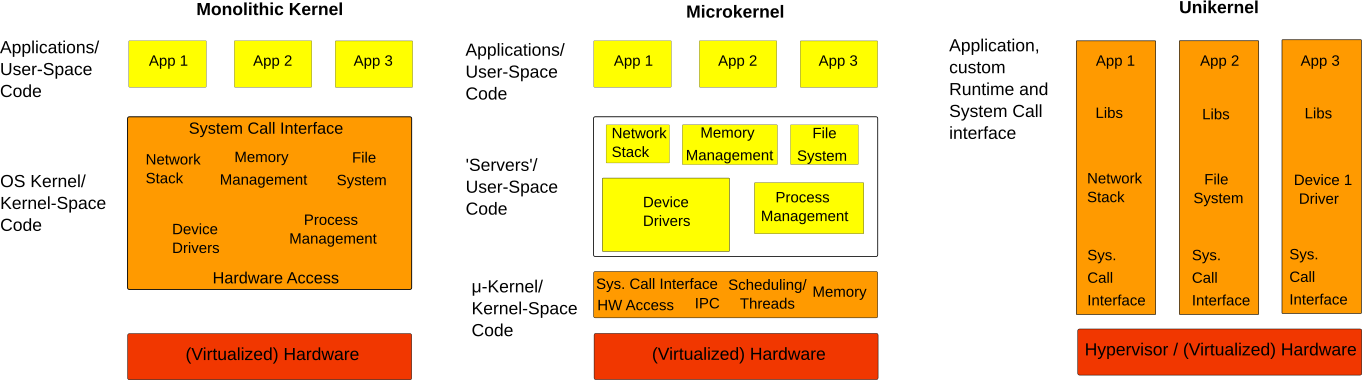
\includegraphics[scale= 0.36]{figures/kernels.png}
    \caption{Structural comparison of Monolithic, Micro- and Unikernels }
    \label{fig:kernels}
\end{figure}

\textbf{Microkernel$\blacktriangleright$} Microkernels follow a \textit{minimality principle} formulated by Liedtke~\cite{jochen1995mu} as \\

\emph{''More precisely, a concept is tolerated inside the $\mu$-kernel only if moving it outside the kernel, i.e. permitting competing implementations, would prevent the implementation of the system's required functionality.''}\\

The central motivation for microkernels, is the reduction of privileged, low-level code executing in kernel mode. Based on the insight, that large code bases of monolithic kernels com e at the costs of large potential for bugs in privileged, low-level (and therefore hard to check) code concepts to minimize kernels and therefore attack surface date back to the 70$^th$ \cite{hansen1970nucleus}. Concepts like the Mach kernel \cite{accetta1986mach}, separation kernels\cite{rushby1981design} or isolation kernels \cite{whitaker2002scale} where developed to minimize and isolate kernel space code, to increase security and enable verification.  

The minimality principle basically limits the essential components of kernel to memory management (i.e. providing access and access control to address spaces), CPU allocation (i.e. providing access to the CPU in any form of process or thread abstraction and scheduling) and inter-process communication (IPC). Other services as I/O, device drivers, networking and others run as userland processes although there might be further distinctions from actual user processes. In addition to the advantage of the smaller attack surface, the low memory requirement also makes microkernels advantageous, especially for embedded systems. 

This design comes with an inherent performance penalty. In a monolithic system a userspace application requiring access to hardware or system services would cause a single context switch to kernel mode. The request would be answered and the result returned to the userspace process. In a microkernel on the other hand, the request of the user application will be forwarded by the kernel via IPC e.g. to a driver process, who again answers via IPC indirected through the kernel. In this simple scenario the number of context switches doubles from two to four. Also the communication among system services is just function calls in monoliths while it again involves IPC and four context switches for each invocation among services. 

Currently existing examples of microkernels are L4 (formerly L3 \cite{liedtke1993persistent}), Minix \cite{herder2006minix}, Singularity \cite{hunt2005overview} or the QNX microkernel OS\cite{hildebrand1992architectural} used in embedded systems for example in phones, or as real time OSs in cars.

\textbf{Unikernels\cite{madhavapeddy2014unikernels} $\blacktriangleright$}: Unikernels also tackle the problem of large code base and attack surface in monolithic kernels. However they follow another approach concerning process isolation. The 'uni' in unikernels refers to the idea of compiling a specific kernel for each application or even component of larger applications.  
tackle single purpose, specialized OS kernels; written in a high-level language; act as individual, potentially distributed components of a full application/software \means the hypervisor controls eg. unikernels for file system, network stack and user process instead of VMs running all those together \means full scaling control is shifted to the hypervisor level, only required resources are scaled


\begin{itemize}
    \item[libOSs]: Unikraft~\cite{kuenzer2021unikraft}, IncludeOS~\cite{bratterud2015includeos}, Graphene~\cite{tsai2014Graphene}
    \item[unikernels]:
\end{itemize}


\todo[inline]{What kind of organization is unikernel.org? \cite{unikernelorg}}
Examples of this are CubicleOS~\cite{sartakov2021cubicleos}, FlexOS~\cite{lefeuvre2021flexos} and M$^3$x~\cite{Asmussen:M3x}, M$^3$v~\cite{Asmussen:M3v}.
\todo[inline]{read \cite{madhavapeddy2014unikernels},CubicleOS~\cite{sartakov2021cubicleos}, FlexOS~\cite{lefeuvre2021flexos} and M$^3$x~\cite{Asmussen:M3x}, M$^3$v~\cite{Asmussen:M3v} \means how are the kernels compiled, what's there scope? }


\textbf{Library Operating Systems}: actually provide the basis for compiling Unikernels; library operating systems provide functionalities of monolithic kernels as independent library implementations e.g. device drivers for physical NICs are implemented in libraries that can be combined with potentially different implementations of the TCP/IP stack. 'MirageOS' is a library operating system.

\section{Our target Backend $M^3$:}
\subsection{The Concept}
\begin{itemize}
    \item M$^3$ is a micro kernel concept/architecture for distributed and potentially heterogeneous architecture
    \item for example as embedded system in mobile devices
    \item it's based on a hardware-OS-co-design approach i.e. specialized HW components for special OS tasks (or the other way around) e.g. separate chips for broadband communication, signal processing (camera, GPS), maybe crypto per device.
    \item specialty of the HW design \means HW components 'tiles' are connected via Trusted Communication Units (TCUs)
    \item the actual (micro) kernel runs on one tile and is the only component privileged to establish communication among other tiles via the TCUs
\end{itemize}
detailed
\begin{itemize}
    \item system architecture to integrate heterogeneous 'compute units' 
    \item CU: computing units with pot. different ISAs e.g. general purpose CPUs, FPGAs, DSPs, fixed-function accelerators
    \item Operating system should let each CU: 
    \begin{itemize}
        \item work independently + isolated (in the security sense)
        \item switch context\means Kernel can schedule other tasks on a CU and swithc them for better HW utilization
        \item communicate directly to each other i.e. no central CPU
        \item access OS services like file system and network stack
    \end{itemize}
    \item How: 
    \begin{itemize}
        \item DTUs: data transfer units are a HW component M§ introduces as common interface at each CU, this allows coherent access to/from the OS
        \item OS Kernel runs on a dedicated CU, controlling the other services 'remotely' via their DTUs 
        \item Context switching means, switching from the execution of one program/ call to another 
        \item Activity: A running entity on a CU, for CPU generally a system thread
        \item Communication with suspended activities (A \means B, B is suspended): So called fast-path communication i.e. communication directly among two Activities without involving the kernel is default. Activities are not aware if their communication partner is currently running or suspended i.e. context was switched by kernel. The lazy approach taken by M3(x) means, the HW detects attempts to communicate with a not-running Activity and errors back to the sending activity. Upon such error, the sending activity A invokes the kernel to schedule B and asserts delivery of message. 
        \item Idle Notification: when activities idle they notify the kernel, which can then schedule another activity
        \item to efficiently schedule an application with many "heavily communicating" activities, a \textbf{Gang schedule} mechanism can be used  by defining the 'gang' of an activity at creation time (?). \means we might use this 
        \item Accelerators: There's two types of them considered 1) request processing accelerators (get a blob of data \means process \means return) 2) stream processing accelerators (get a file/source \means stream process data to a sink). There's ASM (Accelerator Support Module) for both \means not sure we'll need to know this
        \item OS Services - File Access: implemented as 'microservice-style servers', applications and accelerators are clients, access to files via \code{next_in} and \code{next_out} i.e. client (accelerator) requests input and output source, gets \code{next_in} and \code{next_out} and infos on the offset and can retrieve data from/write output to memory using this info without asking the server again. The server has no direct control what is read/written \means follow up requests are considered 'commits' on the previous sections being processed completely \means \textbf{Can/Do we keep that promise? Is it by design or does the software have to comply explicitly?}
    \end{itemize}
    \item Implementation: 
    \begin{itemize}
        \item kernel tile \means runs micro kernel, controls DTUs of 'everybody'
        \item user tiles \means run activities, send sys calls as messages to the kernel, by default they are disconnected from each other
        \item each activity has it's own address space and capabilities, capabilities can be shared via sys calls
        \item system services implemented as servers \means eg. m3fs file system similar to UNIX but grant direct access via DTU, pipe server establishing \textbf{ unidirectional, first-in-first-out communication channel} between activities
        \item context switches \means  placement/scheduling decision by kernel, state of suspended activity saved locally by special component on each user tile (remotely controlled time multiplexer (RCTMux), for general purpose CPUs they are just software), state of DTU (i.e. access rights and channels) stored by the kernel for security reasons, messages for suspended activities are redirected to and buffered by the kernel until rescheduling of the recipient
        \item addressing and forwarding messages: messages have sender and receiver IDs, if a DTU notices $receiverID != currentID$, it errors to $senderID$ so the sender can forward the message to the kernel instead
        \item messages have only-once semantic, data-access can/must be repeated during execution/upon failure
        \item the M3x standard library wraps the \code{next_in}, \code{next_out}, \code{commit} and \code{search} file server communication in a UNIX like API for file access 
        \item file system access for accelerators is implemented in HW, input and output stream (for streaming accelerators) consist of a message and a data channel each
    \end{itemize}
\end{itemize}
\means seems we have (according to design) loss-less communication in order and preemptive scheduling and tasks go idle upon receiving \means looks good concerning our assumptions. 
\todo[inline]{There are different platforms to simulate/host/run M3. Maybe describe them here or in the benchmark section.}

\subsection{The Rust API}
Any backend integration for Ohua needs to specify the implementation for two core primitives of Ohuas DFG language, namely an implementation for the nodes of the Data Flow Graph and an implementation for the edges i.e. the communication channels both following the assumptions of the programming model as described in Section~\ref{sec:back_ohua}. M3 provides a Rust integration to access its abstractions of processes and channels. We will now describe the main features of this API. \\
\todo[inline]{ Maybe extend this description later to really cover the basic features}

To run processes in M3, one first needs to instantiate at least one \rust{Tile}\todo[inline]{lookup struct}. Tiles are M3 abstraction of computing units. Processes running on tiles are called \rust{activity}\todo[inline]{lookup struct}. So we can choose to instantiate the nodes of the DFG as \rust{activity} on the same or different tiles
\todo[inline]{What have we chosen}. To pass initial data to an activity, the attribute \rust{activity.sink()} can be used to serialize data into the process memory. This data can be accessed from inside the activity code using \rust{activity.source()}. Serialization is done using \code{serde} \question]{couldn't find ... ask Nils again}
This is necessary e.g. when a parent process needs to pass some process state to a child process as each activity is spawned i.e. starts without inheriting anything from the parent. \question{Ask Nils: Activities are started as closures. So do we need that source-sink mechanism for imports, consts etc or only for runtime stuff from the main?}. As shown in Figure~\ref{fig:startingActivity} activities are created as closures just as normal threads in Rust. They also mimick the behaviour of normal Rust threads regarding their interfaces for starting them using \code{run}, terminating them using \todo[inline]{Insert terminate call}. They are terminated and their memory is cleaned automatically as soon as they go out of scope.\\ 

\todo[inline]{Figure showing Code for an activity}
\begin{figure}
    \centering
    \begin{minted}{rust}

// Code for starting activity goes here
    
    \end{minted}
    \caption{Creating and running a Rust activity on M3}
    \label{fig:startingActivity}
\end{figure}

Concerning process communication, M3 provides different mechanisms, mainly depending on the size of data to be transmitted. \todo[inline]{Check the other ones when Nils is back}. M3 manages communication among processes using capabilities. The capability to directly send to or receive from another process is implemented as \rust{Gate}s in the M3 Rust API. Gates are directed one-to-one connections, so there are send gates \rust{SGate} and receive gates \rust{RGate}. Receive gates are instantiated with a maximum message size and a maximum overall size of the message buffer to prevent memory overflows in limited environments. The absolute (system immanent) maximum message size is 2 kb. A selector, i.e. an ID of those gates must be delegated to the activities explicitly. Any connection among activities, even on the same tile has to be permitted by the kernel tile and registered at the DTUs of the tiles on which the activities run. This happens automatically for sending gates when the first message is send, but has to be done manually by calling \rust{activate} on the gate handle. \\
\todo[inline]{Check: "Mit dem Selektor muss ein neues Gate in der Activity instantiiert und gebunden werden"}

Sending messages is straight forward as known from most pipe like interfaces. Receiving is done in two steps. First a receive stream is requested using \rust{let stream = rgate.recv_msg()}. This is a blocking call, that will return upon available  messages arriving at the gate. The second step is calling \rust{let msg = stream.pop()} which is non blocking. This call can be done arbitrarily often on an existing stream but will fail if there are no more messages in the stream. Another special feature of the M3 gates is the forcing of a credit system. To prevent too many messages from being sent, the sender requires one credit for each message. To get the credit back after sending a message, the receiver must reply to the message using \rust{reply_vmsg!(/*arbitrary list of reply items*/)} and the sender must receive this reply. Per received reply, the sender will regain one sending credit. It is possible when creating the gates to specify a number of messages that may be sent before new credits are required. The mechanism is similar to the window size in TCP. However, in the end there must be a credit for each message and it is not possible to initialize a send gate e.g. with an arbitrary number of credits. So contrary to the existing integrations, we will have to implement a bidirectional mechanism of message receipt.\\

Finally a limitation of the current M3 API is that the standard library is not supported. There is a separate implementation of \rust{std} with essential functions but partly different function signatures. For smoltcp itself this limitation is not relevant, since it is written without using the standard library. In contrast, the libc API is a necessary part of smoltcp and is supported by M3. 

\subsection{Exisiting M3 Architecture Integration}


\section{smolTCP}
smolTCP~\cite{smolTCP} is a Rust-based open-source implementation of a TCP/IP stack. It runs entirely as a user space application. It also provides conditional compilation features to build applications without heap allocation. This makes smoltcp and applications build with it amenable be used in microkernels as M$^3$\cite{Asmussen:M3v} and embedded systems such as ARTIQ (e.g. \cite{lam2021combining}). In fact the microkernel operating system Redox\cite{redoxwebsite}, as well as M3 itself already use smoltcp for their network stack implementation. So in both systems, smoltcp is used to create a network stack as a sequential, userspace service. This means that, in contrast to the application to be developed in this thesis, the TCP/IP layer, the actual network layer or system interface and the user application communicate with each other via shared memory. \\

The design of the library is structured according to typical TCCP/IP layering. We will briefly introduce the three main layers, or components respectively, that are relevant in this work\footnote{For more information see the documentation at \url{https://docs.rs/smoltcp/latest/smoltcp/}}.


The \code{socket} module provides different socket abstractions implementing the TCP, UDP, IGMP or DHCP protocols respectively as well as for raw sockets. Common features of all those abstractions are keeping track of inbound and outbound data in socket buffers and implementing functionality to package or unpack those data according to the implemented protocol. The sockets keep also track of additional state information, relevant for their respective protocol e.g. TCP or DHCP client states, hop limits, window sizes etc..\\

The \code{iface} module provides the abstractions of the Ip layer. The most important structure is \rust{ Interface}. In an inner component of the interface (\rust{InterfaceInner}) the state data of the IP layer are stored. This includes the IP address of the interface, a routing table, a neighbor cache and the hardware address (depending on the transport medium according to Ethernet or IEEE 802.15.4 standard). Accordingly, the generation and interpretation of IP headers for outgoing and incoming packets are also tasks of the 
\rust{InterfaceInner}. In the currently official variant of smoltcp, the Interface also contains a field \code{Device}, holding an abstraction of the physical network layer, and a \code{SocketSet} to manage all sockets belonging to the interface. Smoltcp is under ongoing development and so in the recent implementation state, \rust{Device} and \rust{Sockets} are no longer part of the interface, but independent structures passed to it to process packets from sockets to device and vice-versa. We will discuss the implication of this in further detail in the Section~\ref{sec:ImplSmoltcp}. \\

Finally the physical layer is implemented in the \rust{phy} module. It provides different implementations of the \rust{Device} trait, to connect the application to the underlying operating systems loopback or tuntap interface or raw sockets. Implementors of the \rust{Device} trait provide the methods \rust{receive}, \rust{transmit} and \rust{capabilities}.\\

The actual transfer of packets from the interface to the device is realized via sending and receiving tokens. We explain in a little more detail here, because it exemplifies a characteristic of the smoltcp code. A successful call to \rust{device.receive()} will yield a tuple of a receive toke \rust{RxToken} and a send token \rust{TxToken}. The former will contain the actual received content as a private field, the later contains a reference to the device specific storage for outgoing packets. In case of tuntap and rawsocket devices, this reference is a file pointer provided by the operating system. In Figure~\ref{fig:TokensAndClosures} the implementation of a sending \rust{TxToken} for raw sockets and the usage of such token to send an Ethernet frame are shown. Two things become apparent. First, the memory for the packets is allocated only at device level upon consuming a token. Second, any structs needed to construct the frame are instantiated in a closure passed as an argument to \rust{tx_token.consume()}. As closures are realized via fixed size structs on the stack frame of the called function, this technique enables smoltcp to work without heap allocation and is used heavily in the code. This principle is used in a cascading manner i.e. \rust{dispatch_ethernet} itself also receives a closure capturing objects from the calling scope.\\

Obviously one implication of separating the layers of smoltcp to different, memory separated components is, that this kind of memory efficiency can not be maintained. 
\todo[inline]{Check and augment link to implementation/discussion section when available}

\begin{figure}[H]
\centering
\tabskip=0pt
\valign{#\cr
    \hbox{%
    \begin{subfigure}{.37\textwidth}
    \centering
     \begin{minted}[fontsize=\tiny]{rust}
// Sending Token for RawSocket

pub struct TxToken {
    lower: Rc<RefCell<sys::RawSocketDesc>>,
}

impl phy::TxToken for TxToken {
    fn consume<R, F>(
    self, 
    ..., 
    f: F) -> Result<R>
    where
        F: FnOnce(&mut [u8]) -> Result<R>,
    {
        let mut lower = self.lower.borrow_mut();
        let mut buffer = vec![0; len];
        let result = f(&mut buffer);
        match lower.send(&buffer[..]) {
            Ok(_) => result,
            // Error handling 
        }
    }
}
     \end{minted}
    \end{subfigure}%
  }
  \cr
  \noalign{\hfill}
    \hbox{%
    \begin{subfigure}{.62\textwidth}
    \centering
    \begin{minted}[fontsize=\tiny]{rust}
    //Interface using a TxToken to send a frame
    
    pub fn dispatch_ethernet<Tx, F>(
    &mut self, 
    tx_token: Tx, 
    buffer_len: usize, 
    f: F) -> Result<()>
    where
        Tx: TxToken,
        F: FnOnce(EthernetFrame<&mut [u8]>),
    {
        let tx_len = EthernetFrame::<&[u8]>::buffer_len(buffer_len);
        tx_token.consume(self.now, tx_len, |tx_buffer| {
            ...
            let mut frame = EthernetFrame::new_unchecked(tx_buffer);
            let src_addr = {...};
            
            // closure from outer scope:
            f(frame);
            Ok(())
        })
    }
    \end{minted}
    \end{subfigure}%
  }
  \vfill
  \cr
}
\caption{Sending and receiving packages is implemented via Tokens exposing a \rust{consume} method, taking closures as argument that process the send or received content. This way, memory allocation can be constrained a) to the device layer and b) to the stack if necessary}
\label{fig:TokensAndClosures}
\end{figure}



\section{Rust}
\todo[inline]{Not sure if I'll need this but collect some infos e.g. closures and the heaplessness of smoltpc at least so I know what the implications are}
\textbf{Closures}: Closures are used in smotcp quite a lot so its important to understand how this influences state sharing and control flow in the original architecture.
\begin{itemize}
    \item if not explicitly annotated, the closure will derive if captured objects are mut/immut borrowed or moved 
\end{itemize}
\begin{minted}{rust}
let obj1 = OBJ1::new();
let closure1 = |arg| {let x =obj1.do_stuff(arg);
                      x*2}
// closure1 is moved to use_closure, 
// while obj2 gets a mutable reference to obj1
obj2.use_closure(closure1);
\end{minted}

Features of Rust that might become relevant for implementation
\begin{itemize}
    \item Type Inference: Rusts type inference is based on standard Hindley-Milner (HM) type inference algorithm\footnote{Full description can be found in \href{https://rustc-dev-guide.rust-lang.org/about-this-guide.html}{the Guide to Rustc Development}}. To resolve trait bounds a Unification algorithm similar to the algorithm used in Prolog to solve logical constraints\footnote{The Trait Bound Unification is implemented in the \href{https://rust-lang.github.io/chalk/book/}{Chalk} library}.
    \todo[inline]{If needed and time allows check (reasons for) limitations and give details on extensions}
    \item Generic Types: To allow the use of generic types with basically no runtime overhead, Rust uses so called \textit{monomorphization} at compile time. This process infers concrete typing for any use of generically typed elements, like functions, structs or enums. The concretely typed instances of elements are then inlined to the existing code. It is in fact one of the last steps on a Rust IR before the code is lowered to LLVM IR and passed to LLVM for code generation and enables LLVM to infer some lower level optimizations (city rustc guide again? ).
    \item Serialization: There is a crate \href{https://doc.rust-lang.org/nightly/nightly-rustc/rustc_serialize/index.html}{serialize}, that as described in the 
\end{itemize}


\subsection{Existing Rust Integration}

\label{subsec:RustIntegration}
Currently supported (working) subset
\begin{table}[H]
    \resizebox{\columnwidth}{!}{%
    \begin{tabular}{l c l l}
        \multicolumn{4}{l}{\emph{Block of Statements:}}\\
        $block$ & $::=$ & \textbf{\{}$s;~\ldots ;~s $\textbf{\}} & statements \\
        \multicolumn{4}{l}{\emph{Statements:} }\\
        $s$ & $::=$ & $ e $ & statement returning a value\\
        & $|$ & $ e $\textbf{;} & statement not returning a value\\
        & $|$ & \textbf{let} $pat$ \textbf{=} $e$ & local definition\\ 
        
        \multicolumn{4}{l}{\emph{Expressions:}}\\
        $e$ & $::=$ & $x$ & variable bindings \\
        & $|$ & $\textbf{1},\textbf{2},\textbf{3}, \ldots \ |\ \textbf{true}\ |\ \textbf{false}\ $  & literals \\
        & $|$ & $e$ \textbf{(}$e, \ldots , e$\textbf{)} & function calls \\
        & $|$ & $e$ $callRef$ \textbf{(}$e, \ldots , e$\textbf{)} & method calls \\
        & $|$ & $\textbf{(} e,~\ldots ,~e \textbf{)}\ $ & tuples\\
        & $|$ & $e\ +\ e\ |\ e\ -\ e \ |\ e\ > \ e\ |\ e\ == \ e\ |\ \ldots $ & binary operations \\
        & $|$ & $ -e\ |\ !e\ |\ *e\ $ & unary operations\\
        & $|$ &\textbf{if} $e$ $block$ \textbf{else} $e$& conditional with optional else branch \\
        % & $|$ & \textbf{while} $\ e$  $block$ & \\ % actually while loops are not supported at all
        & $|$ & \textbf{for} $pat$ \textbf{in} $e$ $block$ & \\ 
        & $|$ & \textbf{move} $\textbf{| } arg,~\ldots ,~arg \textbf{ |}\ e$ & closure\\
        &$|$& $block$ & block expression, i.e. block returning a value\\
        \multicolumn{4}{l}{\emph{Call References:}}\\
        $callRef $ & $::=$ & $ z\textbf{.}y\textbf{.}x$ $[gernericArg]$  & namespaced binding  \\
        \multicolumn{4}{l}{\emph{Patterns:}}\\
        $pat$ & $::=$ & $x\ |\ (x,~\ldots ,~x)|\ \_ $ & bindings, tuples or wild cards \\
    \end{tabular}%
    }
    \caption{Subset of Rust grammar, that is accepted by the integration frontend}
    \label{tab:FESubset}
\end{table}

